\scanpage{3}
Conversations avec Deligne du 30.5 et 5.6.
\margin{\unsure{i}}

1) Pour groupes finis opérant sur surfaces : utiliser ``th de Smith'' (contre \unsure{patholog}) pour prouver que \unsure{les} ens des points fixes \unsure{est une} variété homologique du pt de vue local -- donc si \unsure{dim 1} loc. connexe, donc connexe par arcs...

2) Exemple de Bing d'une involution de $B^3$ ayant un \unsure{ens} de pts fixes sauvage (\inserted{\unsure{genre}} sphère d'Alexander) mais dont la restriction à $S^2=\partial B^3$ est la conj. complexe.

3) Il doit y avoir des actions \inserted{\unsure{différentiables}} de groupes finis sur $B^n$ ($n\geq\deleted{\unsure{3\ 4}}\ 5$ ?) qui ne sont pas le cône d'une action sur $S^{n-1}=\partial B^n$. Lié au fait qu'une action \deleted{\unsure{linéaire} \illegible{1}} d'un groupe fini sur une sphère \deleted{\unsure{ce disque} \illegible{3}} \inserted{avec pt fixe} n'est pas \unsure{néc\textsuperscript{t}} contenue dans un conjugué \inserted{topologique} du groupe orthogonal. (J'ai pas bien compris comment...)

4) Nécessité de faire intervenir la forme \unsure{intersect.} (à valeurs dans $\unsure{T}$) pour décrire \deleted{la \unsure{forme}} structure ``arithmétique'' du groupe fondamental d'une courbe lisse propre connexe sur $k$ \unsure{alg.} clos. Question de définir algébriquement les intersections de ``chemins'' (au sens théorie des revêtements)

\figure{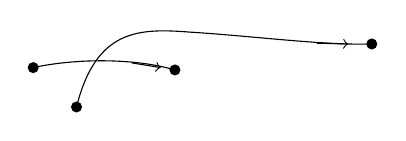
\begin{tikzpicture}[x=1cm,y=1cm]
\fill (0,0) circle (2pt) (1.8,-.03) circle (2pt) (.55,-.5) circle (2pt) (4.3,.3) circle (2pt);
\draw (0,0) .. controls (.55,.12) and (1.3,.12) .. (1.8,-.03);
\draw[->] (1.25,.06)--(1.62,0);
\draw (.55,-.5) .. controls (.8,.5) and (1.35,.5) .. (2,.45) .. controls (2.8,.4) and (3.7,.28) .. (4.3,.3);
\draw[->] (3.6,.31)--(4,.3);
\end{tikzpicture}}

Donner théorie cohomologique d'une courbe dans le \unsure{prodisque|prodiscret}

......

\figure{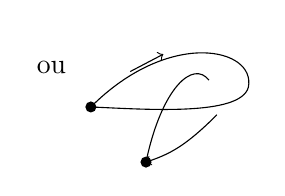
\begin{tikzpicture}[x=1cm,y=1cm]
\node at (-.5,.5) {ou};
\fill (0,0) circle (2pt) (.7,-.7) circle (2pt);
\draw (0,0) .. controls (1,1) and (2.1,.75) .. (2,.25) .. controls (1.9,-.12) and (.7,-.03) .. (0,0);
\draw[->] (.5,.45)--(.92,.67);
\draw (.7,-.7) .. controls (.9,.25) and (1.3,.6) .. (1.5,.34);
\draw[->] (1.6,-.1) .. controls (1.2,-.5) and (1,-.6) .. (.7,-.7);
\end{tikzpicture}}
\figure{\begin{tikzpicture}[x=1cm,y=1cm]
\node at (-.8,1.2) {ou};
\fill (0,.5) circle (2pt) (.9,.9) circle (2pt) (1.1,-.7) circle (2pt);
\draw (0,.5) .. controls (1.3,2) and (1.6,1.4) .. (1.15,.65) .. controls (.8,.3) and (.3,.45) .. (0,.5);
\draw[->] (.72,.45)--(.35,.45);
\draw[->] (.9,.9) .. controls (.83,.1) and (1,-.35) .. (1.1,-.7);
\end{tikzpicture}}

\mspage{2}
